% Horizon penetrating coordinates (vs. Schwarzschild coordinates)
% for a black hole spacetime, with excision
% Author: Jonah Miller
\documentclass[tikz,border=6pt]{standalone}
\usepackage{tikz}
\usetikzlibrary{arrows}
\usetikzlibrary{arrows.meta}
\usetikzlibrary{decorations.markings}
\usepackage{pgfplots}

\tikzset{>={Latex[length=3mm]}}

\begin{document}
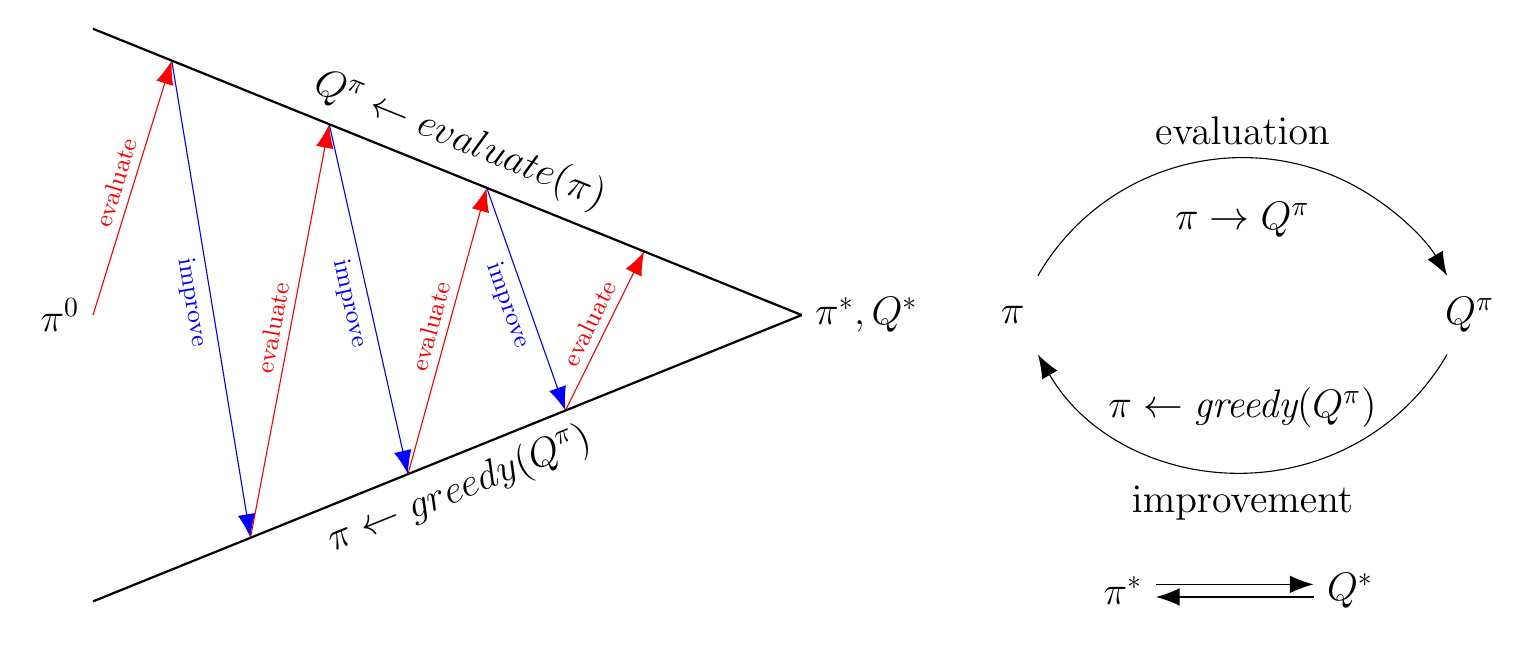
\begin{tikzpicture}
\Large
\draw[-] (0,0) node[left]{$\pi^0$};
\small

\def\angle{22}

\draw[->,red] (0,0)-> (1,{8*tan(\angle)}) node[midway,above,sloped]{evaluate};
\draw[->,blue] (1,{8*tan(\angle)}) -> (2,{-7*tan(\angle)}) node[midway,below,sloped]{improve};
\draw[->,red] (2,{-7*tan(\angle)}) -> (3,{6*tan(\angle)})node[midway, above,sloped]{evaluate};
\draw[->,blue] (3,{6*tan(\angle)}) -- (4,{-5*tan(\angle)})node[midway,below,sloped]{improve};
\draw[->,red] (4,{-5*tan(\angle)}) -- (5,{4*tan(\angle)})node[midway, above,sloped]{evaluate};
\draw[->,blue] (5,{4*tan(\angle)}) -- (6,{-3*tan(\angle)})node[midway,below,sloped]{improve};
\draw[->,red] (6,{-3*tan(\angle)}) -- (7,{2*tan(\angle)})node[midway, above,sloped]{evaluate};


\Large
\draw[-,thick] (0,{9*tan(\angle)}) -- (9,0) node[midway, above,sloped]{$Q^\pi\gets evaluate(\pi)$};
\draw[-,thick] (0,{-9*tan(\angle)}) -- (9,0) node[midway,below,sloped]{$\pi \gets greedy(Q^\pi)$};

\draw[-] (9,0) node[right]{$\pi^*, Q^*$};
\Large
\draw[-] (12,0) node[left]{$\pi$};
\draw[-] (17,0) node[right]{$Q^{\pi}$};

\draw[->] (12,0.5) arc (150:30:3) node[midway,below=0.4cm]{$\pi\rightarrow Q^{\pi}$} node[midway,above]{evaluation};
\draw[<-] (12,-0.5) arc (-150:-30:3) node[midway,below]{improvement} node[midway,above=0.4cm]{$\pi\gets \textit{greedy} (Q^\pi)$};

\Large
\draw[] (13.5,-3.5) node[left]{$\pi^*$};
\draw[] (15.5,-3.5) node[right]{$Q^*$};
\draw[->] (13.5,-3.42) -- (15.5,-3.42);
\draw[<-] (13.5,-3.58) -- (15.5,-3.58);

\end{tikzpicture}
\end{document}